\documentclass{simcenterdocumentation}
\usepackage{amsmath,amssymb}
\usepackage{mathtools}
\usepackage{biblatex}
\usepackage{amsthm}
\usepackage{mathtools}
\usepackage{cases}
\usepackage{booktabs}
\usepackage{multirow}
\usepackage{graphicx}
\usepackage{subcaption}
\usepackage{appendix}
\usepackage{color}
\usepackage{hyperref}
\usepackage{array}
\usepackage{float}
\usepackage{booktabs}
\usepackage{adjustbox}

% To compile this file, run "latex/pdflatex EBD-documentation", then "biber EBD-documentation"
% (or "bibtex EBD-documentation", if the output from latex asks for that instead),
% and then "latex/pdflatex EBD-documentation" (without the quotes in each case).

% Double spacing, if you want it.  Do not use for the final copy. Can also specify
% draft as a document class option. This will generate double spacing and placeholders
% for title page and header images
%% \def\dsp{\def\baselinestretch{2.0}\large\normalsize}
%% \dsp

\usepackage{listings}
\usepackage{color}

\definecolor{dkgreen}{rgb}{0,0.6,0}
\definecolor{gray}{rgb}{0.5,0.5,0.5}
\definecolor{mauve}{rgb}{0.58,0,0.82}
\definecolor{lightgrey}{rgb}{0.95,0.95,0.95}
\definecolor{darkgrey}{rgb}{0.50,0.50,0.50}

\lstset{
  frame=shadowbox, 
  language=C,
  aboveskip=3mm,
  belowskip=3mm,
  showstringspaces=false,
  columns=flexible,
  basicstyle={\small\ttfamily},
  numbers=none,
  numberstyle=\tiny\color{gray},
  keywordstyle=\color{blue},
  commentstyle=\color{dkgreen},
  stringstyle=\color{mauve},
  breaklines=true,
  breakatwhitespace=true,
  tabsize=3,
  rulesepcolor=\color{darkgrey},
  backgroundcolor=\color{lightgrey}
}

\graphicspath{%
              {figs},%
	      {images/},%
	      {theory},%
	      {theory/figs}%
	     }

%%%%%%%%%%%%%%%%%%%%%%%%%%%%%%%%%%%%%%%%%%%%%%%%%%%%%%%%%%%%%%%%%%%%%%%
%
% gloabal layout settings
%
%%%%%%%%%%%%%%%%%%%%%%%%%%%%%%%%%%%%%%%%%%%%%%%%%%%%%%%%%%%%%%%%%%%%%%%

%
% paragraph layout
%
% \parindent	0pt
% \parskip	3pt plus2pt minus1pt
%
% border width of fbox
%
\fboxsep	10pt
\fboxrule	1pt
%
% placement of floats
%
\def\topfraction{0.95}
\def\bottomfraction{0.95}
\def\textfraction{0.05}

%%\setcounter{topnumber}{1}
%%\setcounter{bottomnumber}{1}
%
% debug messages
%
%%\hfuzz 1pt

%%%%%%%%%%%%%%%%%%%%%%%%%%%%%%%%%%%%%%%%%%%%%%%%%%%%%%%%%%%%%%%%%%%%%%%
%
% gloabal abbreviations
%
%%%%%%%%%%%%%%%%%%%%%%%%%%%%%%%%%%%%%%%%%%%%%%%%%%%%%%%%%%%%%%%%%%%%%%%

%
% where to find global definitions
%
\def\TeXDIR	{./TeX/}

%
% load glocal abbreviations file
%
% \usepackage{times,mathptm}
% \usepackage{\TeXDIR PSshort}
%\include{\TeXDIR kurz}

%
% layout style definitions
%
\def\DS{\displaystyle}
\def\TS{\textstyle}
\def\SS{\scriptstyle}

%%%%%%%%%%%%%%%%%%%%%%%%%%%%%%%%%%%%%%%%%%%%%%%%%%%%%%%%%%%%%%%%%%%%%%%
%
% definition of new environments
%
%%%%%%%%%%%%%%%%%%%%%%%%%%%%%%%%%%%%%%%%%%%%%%%%%%%%%%%%%%%%%%%%%%%%%%%

% \newcounter{cremark}
% \def\theremark{\arabic{cremark}}
\newcounter{cremark}[section]
\def\theremark{\thesection.\arabic{cremark}}

\newcounter{ctable}
\newenvironment{mybox}{%
                         \localeqn
			 \setcounter{ctable}{\value{table}}%
			 \refstepcounter{ctable}%
		         \def\theequation{\roman{equation}}%
		         % \def\theequation{\arabic{ctable}-\roman{equation}}%
			 \begin{minipage}[c]{0.95\hsize}%
			}%
                        {\par\end{minipage}%
			 \globaleqn\medskip}  
                        % {\hfill$\bullet$\par\medskip}  
\newenvironment{rem}{%
                         \refstepcounter{cremark}%
                         %\localeqn
		         %\def\theequation{\alph{equation}}%
			 \par
                         \penalty-1000
                         \medskip
                         \noindent
                         {\textbf{Remark~\theremark:}}%
                         % \penalty 10000
			 \leavevmode
			 \textsl\bgroup
			}%
                        {\egroup\par
			 %\globaleqn
			 \medskip}  
                        % {\hfill$\bullet$\par\medskip}  
\newcounter{saveequation}
\def\localeqn{\setcounter{saveequation}{\value{equation}}%
              \setcounter{equation}{0}%
	      \let\savetheqn\theequation}
\def\globaleqn{\setcounter{equation}{\value{saveequation}}%
               \let\theequation\savetheeqn}

%%%%%%%%%%%%%%%%%%%%%%%%%%%%%%%%%%%%%%%%%%%%%%%%%%%%%%%%%%%%%%%%%%%%%%%
%
% local abbreviations
%
%%%%%%%%%%%%%%%%%%%%%%%%%%%%%%%%%%%%%%%%%%%%%%%%%%%%%%%%%%%%%%%%%%%%%%%

\def\vectorform#1{\ensuremath{\left\{#1\right\}}}
\def\matrixform#1{\ensuremath{\left[#1\right]}}

\long\def\putinvector#1{\vectorform{\begin{array}{c}#1\end{array}}}
\long\def\putinmatrix#1{\matrixform{\begin{array}{ccc}#1\end{array}}}

\newcommand{\trace}{\mathop{\mathrm{tr}}}
\newcommand{\sign}{\mathop{\mathrm{sign}}}
\newcommand{\vol}{\mathop{\mathrm{vol}}}
\newcommand{\dev}{\mathop{\mathrm{dev}}}
\newcommand{\norm}[1]{\mathop{\left\Vert#1\right\Vert}}

\def\mathBox#1{\fbox{$\displaystyle #1$}}

\def\R{\mathbb{R}}
\def\N{\mathbb{N}}

%
% number spaces
%
\def\R		{\mathbb{R}}
\def\N		{\mathbb{N}}
\def\Rplus	{\R^+}
\def\Nplus	{\N^+}
\def\Roplus	{\R_0^+}
\def\Noplus	{\N_0^+}

%
% differential operations:
%
% ... total derivative
\newcommand{\diff}[2]{\frac{d #1}{d #2}}
%
% ... second order total derivative
\newcommand{\ddiff}[2]{\frac{d^2 #1}{d #2^2}}
%
% ... mixed second order total derivative
\def\mddiff#1#2#3{\frac{d^2 #1}{d #2\,d #3}}
%
% ... partial derivative
\newcommand{\pdiff}[2]{\frac{\partial #1}{\partial #2}}
%
% ... second order partial derivative
\newcommand{\pddiff}[2]{\frac{\partial^2 #1}{\partial #2^2}}
\newcommand{\ppdiff}[3]{\frac{\partial^2 #1}{\partial #2\otimes\partial #3}}
%
% ... mixed second order partial derivative
\def\mppdiff#1#2#3{\frac{\partial^2 #1}{\partial #2\,\partial #3}}

%
% text in formulas
%
\def\AND	{\hbox{and}}
\def\OR    {\hbox{or}}
\def\WITH	{\hbox{with}}

%
% tensor operators
%
\def\tr		{\mathop{\mathrm{tr}}}
\def\dev	{\mathop{\mathrm{dev}}}
\def\DEV	{\mathop{\mathrm{DEV}}}
\def\INV	{^{(-1)}}
\def\inv	{^{-1}}
\def\sqr	{^{2}}
\def\qub	{^{3}}
\def\Lie	{\mathcal{L}_v}

%\newcommand{\vectr}[1]{\mathbf{#1}}
\newcommand{\vectr}[1]{{\hbox{\boldmath$#1$}}}
\newcommand{\tensor}[1]{{\hbox{\boldmath$#1$}}}

\newcommand{\Div}{\mathop{\mathrm{Div}}}
\newcommand{\Grad}{\mathop{\mathrm{Grad}}}
\newcommand{\diver}{\mathop{\mathrm{div}}}
\newcommand{\grad}{\mathop{\mathrm{grad}}}
\newcommand{\deter}{\mathop{\mathrm{det}}}

%
% standard symbols
%

%
% special tensors (4th-order)
%
\def\I		{\mathbb{I}}
\def\IC		{\I_\vectr{C}}
\def\ICinv	{\I_{\Cinv}}
\def\Ib		{\I_\vectr{b}}
\def\IMi	{\I_{\stackrel{1}{\vectr{M}}}}
\def\IMii	{\I_{\stackrel{2}{\vectr{M}}}}
\def\IMiii	{\I_{\stackrel{3}{\vectr{M}}}}
\def\IMal	{\I_{\stackrel{\alpha}{\vectr{M}}}}
\def\IMbe	{\I_{\stackrel{\beta}{\vectr{M}}}}
\def\Imi	{\I_{\stackrel{1}{\vectr{m}}}}
\def\Imii	{\I_{\stackrel{2}{\vectr{m}}}}
\def\Imiii	{\I_{\stackrel{3}{\vectr{m}}}}
\def\Imal	{\I_{\stackrel{\alpha}{\vectr{m}}}}
\def\Imbe	{\I_{\stackrel{\beta}{\vectr{m}}}}

\def\IDEV	{\I^{\textrm{dev}}}
\def\Idev	{\left( \I-{\TS\frac{1}{3}}\,\Bone\otimes\Bone \right)}

%
% functions
%
\def\norm#1{\|#1\|}
\def\inpd#1{{<}#1{>}}

\newcommand{\citep}[1]{(\cite{#1})}




\bibliography{references}

\begin{document}
% Declarations for Front Matter
% Software title followed by optional second line
\title{EBD\\ \Large Elastic Body Dynamics}
% Use superscripts to indicate author affiliations
\author{Jiawei Wan$^{1}$, Peter Mackenzie-Helnwein$^2$}
\institutions{$^1$University of Notre Dame \\$^2$University of Washington}
\softwarename{Elastic Body Dynamics}
\softwareversion{1.0.0}

%%% DON'T MESS WITH THESE SETTINGS %%%%%%%%%%%%%%%%%%%%%%%%%%%%%%%%
\hypersetup{pageanchor=false}
\maketitle
\copyrightpage
\acknowledgments

\hypersetup{pageanchor=true}
\begin{frontmatter}

\pagestyle{plain}
{
  \renewcommand{\thispagestyle}[1]{}
  \tableofcontents
  \clearpage
  \listoffigures
  %\clearpage
  %\listoftables
}

\end{frontmatter}
\pagestyle{somewhatsimple}
%%%%%%%%%%%%%%%%%%%%%%%%%%%%%%%%%%%%%%%%%%%%%%%%%%%%%%%%%%%%%%%%%%%
% Create separate tex files for each chapter and provide them as inputs

\chapter{Tool Audience}
%% chapter: Tool Audience

Researchers, students and engineers who are interested in the numerical simulation
of the fluid-structure interaction using the open-source tool box OpenFOAM.




\chapter{Introduction}
%% Chapter: Introduction

The Elastic Body Dynamics Tool (EBD) is designed to collect all required properties and parameters
needed for modeling the aeroelastic behavior of an deformable body immersed in surrounding fluids using the OpenFOAM, and to augment an OpenFOAM model by adding the necessary sections to respective parameter definition files. The generic workflow involved is as follows.

\begin{enumerate}
\item
   Build your OpenFOAM model as you would without using the elastic body dynamics library. 
   
\item
   Run EBD following, identify your model folder, adjust the parameters as desired, and export to your model definition. Consult Chapter~\ref{sec:EBD-theory} for details on those steps.
   
\item
    Run the updated model using the dynamic finite volume mesh solver provided by EBD.
    
\end{enumerate}

\noindent The tool also provides a Save to file and Open from file functionality that will allow you to
define and share complex sets of settings and parameters required by the usage of EBD, such, efficiently and reliably apply the same parameters to several different models.

%% leave this as overview

The following Chapter~\ref{sec:EBD-installation} explains the installation of the tool. Chapter~\ref{sec:EBD-theory} provides a detailed theoretical background and code implementation of the tool.  Chapter~\ref{sec:EBD-usage} summarizes the work-flow and required parameters of the tool. Chapter~\ref{sec:EBD-demonstration} demonstrates two numerical examples on the implementation of the tool.

\chapter{Installation Instructions}
\label{sec:EBD-installation}

\section{Installing the Elastic Body Dynamics Tool}

Download the installation package for your operation system from (a single line)

\begin{verbatim}
https://www.designsafe-ci.org/data/browser/public/designsafe.storage.community/
            /SimCenter/Software/elasticBodyDynamicsTool
\end{verbatim}

SimCenter is providing packages for Windows~8/10 (64 bit version only) and MacOS. The installer will place the executable on your system.  On Windows systems, a shortcut will be added to your start menu. On MacOS, the application is placed in your Applications folder.

\bigskip

For Linux systems, you will need to clone the source from 

\begin{verbatim}
https://github.com/NHERI-SimCenter/elasticBodyDynamicsTool
\end{verbatim}

and compile it yourself performing the following steps:

\begin{quote}
\begin{verbatim}
$ git clone https://github.com/NHERI-SimCenter/elasticBodyDynamicsTool
$ git clone https://github.com/NHERI-SimCenter/SimCenterCommon
$ cd elasticBodyDynamicsTool
$ qmake elasticBodyDynamicsTool.pros
$ make
$ sudo make install
\end{verbatim}
\end{quote}

\section{Compiling the Source Code in OpenFOAM}

Download the source code of the elastic body dynamics library from

\begin{verbatim}
https://github.com/NHERI-SimCenter/elasticBodyDynamicsTool/elasticBodyDynamics
\end{verbatim}

\noindent Note that the code is provided for OpenFOAM version 7. So please install the correct OpenFOAM version following the instructions from

\begin{verbatim}
https://openfoam.org/release/7/
\end{verbatim}

\noindent Create a project directory named as \textcolor{blue}{run} within the \textcolor{blue}{\$HOME/OpenFOAM} directory named \textless{USER}\textgreater{-7} (e.g. SimCenter-7 for user SimCenter and OpenFOAM version 7) by typing the following script in a terminal prompt:

\begin{quote}
\begin{verbatim}
$ mkdir -p $FOAM_RUN
\end{verbatim}
\end{quote}

\noindent Copy or move the \textcolor{blue}{elasticBodyDynamics} directory which has been downloaded earlier and all the files in it to the \textcolor{blue}{\$HOME/OpenFOAM} directory. Go the relocated \textcolor{blue}{elasticBodyDynamics/src} directory by typing:

\begin{quote}
\begin{verbatim}
$ cd $FOAM_RUN/elasticBodyDynamics/src
\end{verbatim}
\end{quote}

\noindent Compile the files in the \textcolor{blue}{elasticBodyDynamics/src} directory by typing the following in the terminal prompt:

\begin{quote}
\begin{verbatim}
$ wmake
\end{verbatim}
\end{quote}

\noindent After the compilation is successfully complete, a library file named as \textcolor{blue}{libelasticBodyDynamics.so} will be generated in the directory \textcolor{blue}{\$FOAM\_USER\_LIBBIN}.

\noindent Go the relocated \textcolor{blue}{elasticBodyDynamics/applications/pimpleFoam} directory by typing:

\begin{quote}
\begin{verbatim}
$ cd $FOAM_RUN/elasticBodyDynamics/applications/pimpleFoam
\end{verbatim}
\end{quote}

\noindent Compile the files in the \textcolor{blue}{elasticBodyDynamics/applications/pimpleFoam} directory by typing the following in the terminal prompt:

\begin{quote}
\begin{verbatim}
$ wmake
\end{verbatim}
\end{quote}

\noindent After the compilation is successfully complete, an application named as \textcolor{blue}{newPimpleFoam} will be generated in the directory \textcolor{blue}{\$FOAM\_USER\_APPBIN}.





\chapter{Theory}
\label{sec:EBD-theory}

\section{Introduction}

This section introduces the use of the elasticBodyDynamics library in the open-source computational fluid dynamics (CFD) code, OpenFOAM. The library is developed for solving the motion of a deformable body subjected to aerodynamic loads in which the body can be modeled as an elastic beam, and transform the dynamic finite volume mesh to cope with the motion of the body. The beam is assumed to have tension, compression, torsion and bending capabilities. It has six degrees of freedom at each point (or node) on the beam: translations in the $x$, $y$ and $z$ directions and rotations about the $x$, $y$ and $z$ axes. Based on theories on structural dynamics, the motion equation of such a beam model can be expressed as 

\begin{equation} \label{motionEquation}
\boldsymbol{M}\ddot{\boldsymbol{Y}}(t)+\boldsymbol{C}\dot{\boldsymbol{Y}}(t)+\boldsymbol{K}\boldsymbol{Y}(t) = \boldsymbol{P}(t)
\end{equation}

\noindent In (\ref{motionEquation}), $\boldsymbol{Y}$ and $\boldsymbol{P}$ represents the vectors of the generalized displacements and (aerodynamic) loads, respectively. $\boldsymbol{M}$, $\boldsymbol{C}$ and $\boldsymbol{K}$ denote the generalized mass, damping ratio and stiffness diagonal matrices with the $i$-th diagonal elements, respectively, given by

\begin{equation}
M_i = \boldsymbol{\phi}_i^T\boldsymbol{m}\boldsymbol{\phi}_i, \quad
K_i = \omega_i^2M_i, \quad
C_i = 2\zeta_i\omega_iM_i
\end{equation}

\noindent where $\boldsymbol{m}$ is the mass matrix, $\omega_n$ denotes the natural frequency of the $n$-th vibration mode and $\boldsymbol{\phi}_i$ stands for a vector storing the shape of the $i$-th vibration mode. Meanwhile, the generalized load associated with the $i$-th mode admits the form

\begin{equation}
P_i(t) = \boldsymbol{\phi}_i^T\boldsymbol{p}(t)
\end{equation}

\noindent where $\boldsymbol{p}(t)$ is the vector of aerodynamic loads. After the solution of the motion equation (\ref{motionEquation}), the overall displacement of the system can be computed from

\begin{equation}
\boldsymbol{v}(t) = \boldsymbol{\varPhi}\boldsymbol{Y}(t)
\end{equation}

\noindent in which

\begin{equation}
\boldsymbol{\varPhi} = \left(\boldsymbol{\phi}_1,\boldsymbol{\phi}_2,...,\boldsymbol{\phi}_n\right).
\end{equation}

The main objectives of the developed elasticBodyDynamics library includes solving the motion equation (\ref{motionEquation}), computing the displacements of the elastic body and updating the dynamic mesh to cope with the relative motion of the body inside the computational domain. The matrices $\boldsymbol{M}$, $\boldsymbol{C}$ and $\boldsymbol{K}$ involved in (\ref{motionEquation}) are determined from $\boldsymbol{m}$, $\zeta$ and $\boldsymbol{\varPhi}$, all of which require the input from users. On the other hand, the fluid solvers available in OpenFOAM are responsible for the computation of $\boldsymbol{p}(t)$ through solving the fluid equations (e.g., the Navier-Stokes equation and the continuity equation) that govern the flow around the elastic body.

\section{Elastic body dynamics library}

In this section, the elasticBodyDynamics library will be explored. For the ease of understanding of the readers, it is divided into two parts, main files and auxiliary files. The main files include the generalizedMotionState, generalizedSolver, generalizedMotion, sixDoFElasticBodyMotion and sixDoFElasticBodyMotion classes. The auxiliary files include the vector6D and binnedForces classes.

\subsection{generalizedMotionState}

The generalizedMotionState class holds the generalized motion state of an elastic body. The generalized motion state of the body includes the generalized displacement, velocity and acceleration, all of which are stored in a list of scalars, respectively. The number of the elements in each list equals to the number of vibration modes considered during the calculation.

\begin{lstlisting}
class generalizedMotionState
{
    // Private data

        //- Generalized displacement of beam
        List<scalar> ubar_;

        //- Generalized velocity of beam
        List<scalar> vbar_;

        //- Generalized acceleration of beam
        List<scalar> abar_;
\end{lstlisting}

\noindent The initial values of the generalized, velocity and acceleration can be entered in a file named as generalizedMotionState (the location of this file will be discussed later) using the keywords ubar, vbar and abar, respectively, as can be seen from the following lines presented in generalizedMotionState.C:

\begin{lstlisting}
Foam::generalizedMotionState::generalizedMotionState
(
    const dictionary& dict
)
{
    ITstream& is = dict.lookup("ubar");
    is >> static_cast<List<scalar>&>(ubar_);

    is = dict.lookup("vbar");
    is >> static_cast<List<scalar>&>(vbar_);

    is = dict.lookup("abar");
    is >> static_cast<List<scalar>&>(abar_);
}
\end{lstlisting}

\subsection{generalizedSolver}

The generalizedSolver class contains several different methods that can be used to solve the motion equation (\ref{motionEquation}). The solvers contained in this class are:

\begin{itemize}

\item Crank Nicholson
\item Newmark
\item Symplectic

\end{itemize}

\noindent  One of these solvers can be chosen according to requirements of the problem to be solved. Such information has to be entered in the dynamicMeshDict dictionary under the solver sub-dictionary. Taking the following lines in Newmark.C for demonstration, 

\begin{lstlisting}
void Foam::generalizedSolvers::Newmark::solve
(
    bool firstIter,
    const List<scalar>& fbar,
    scalar deltaT,
    scalar deltaT0
)
{
    // Update the linear acceleration and torque
    updateAcceleration(fbar);

    // Correct velocity
    vbar() = vbar0() + deltaT*(gamma_*abar() + (1 - gamma_)*abar0());

    // Correct displacement
    ubar() = ubar0() + deltaT*vbar0() + sqr(deltaT)*(beta_*abar() + (0.5 - beta_)*abar0());
}
\end{lstlisting}

\noindent the member function (named as `solver') updates the generalized displacement, velocity and acceleration of the elastic body taking the generalized load, the current and the previous time-step sizes as the input variables.

\subsection{generalizedMotion}

The generalizedMotion class calls generalizedSolver and generalizedMotionState to compute and print the generalized motion state of the elastic body in each time step, as can be seen in the following lines of generalizedMotion.C:

\begin{lstlisting}
void Foam::generalizedMotion::solve
(
    bool firstIter,
    const List<scalar>& fbar,
    scalar deltaT,
    scalar deltaT0
)
{
    if (Pstream::master())
    {
        solver_->solve(firstIter, fbar, deltaT, deltaT0); 

        if (report_)
        {
            Info<< "generalized motion" << nl
                << "    generalized load: " << fbar << nl;

            status();
        }
    }

    Pstream::scatter(motionState_);
}
\end{lstlisting}

\subsection{sixDoFElasticBodyMotion}

The sixDoFElasticBodyMotion class is a derived class of the generalizedMotion class. It is used to create a system of an elastic beam with six degrees of freedom at each node on the beam. The initialization of such a system requires a list of inputs defined in the dynamicMeshDict (more details regarding those inputs are summarized in Table). The beam is established by connecting a set of nodes with line elements. The nodes are located on a line segment based on the origin and spacing (i.e., the variable with the keywords `origin' and `length', respectively) provided by users. Users are also asked to the specify the information (including the mode shape, natural frequency and damping ratio) of all vibration modes involved in the solution the motion equation of the body.

After obtaining the above mentioned information, the sixDoFElasticBodyMotion class then computes the generalized mass, stiffness and damping ratio of the elastic body during the initialization, which can be seen in the following lines of sixDoFElasticBodyMotion.C:

\begin{lstlisting}
Foam::sixDoFElasticBodyMotion::sixDoFElasticBodyMotion
(
    const dictionary& dict,
    const dictionary& stateDict
)
:
    origin_(dict.lookupOrDefault<vector>("origin", Zero)),
    direction_(dict.lookupOrDefault<vector>("direction", vector(0,0,1))),
    nNode_(dict.lookupOrDefault<label>("nNode", Zero)),
    nMode_(dict.lookupOrDefault<label>("nMode", Zero)),
    frequency_(dict.lookup("frequency")),
    dampingRatio_(dict.lookup("dampingRatio")),
    mass_(dict.lookup("mass")),
    length_(dict.lookup("length")),
    gMotion_(dict, stateDict, nMode_)
{
    mode_.setSize(nMode_);

    forAll(mode_, indi)
    {
        word imode(std::to_string(indi+1));
        word modeName("mode"+imode);

        ITstream& is = dict.lookup(modeName);
        is >> static_cast<List<vector6D>&>(mode_[indi]);

        gMotion_.mbar()[indi] = sum(mass_&mode_[indi]);
        gMotion_.kbar()[indi] = gMotion_.mbar()[indi]*
        sqr(constant::mathematical::twoPi*frequency_[indi]);
        gMotion_.cbar()[indi] = 2.0*constant::mathematical::twoPi*
        gMotion_.mbar()[indi]*dampingRatio_[indi]*frequency_[indi];
    }

    Info<< "generalized mass: " << gMotion_.mbar() << nl
        << "generalized stiffness: " << gMotion_.kbar() << nl
        << "generalized damping: " << gMotion_.cbar() << nl
        << "generalized displacement: " << gMotion_.state().ubar() << nl
        << "generalized velocity: " << gMotion_.state().vbar() << nl
        << "generalized acceleration: " << gMotion_.state().abar() << nl
        << endl;
}
\end{lstlisting}

During the simulation, the sixDoFElasticBodyMotion class calculates the generalized load taking the (fluid-induced) forces and moments acting on each individual beam element as the input variables

\begin{lstlisting}
Foam::List<Foam::scalar> Foam::sixDoFElasticBodyMotion::updateGeneralizedForces
(
    const List<vector> forces,
    const List<vector> moments
)
{
    List<scalar> fbar(nMode(), Zero);
    List<vector6D> nodalForces(nNode(), vector6D::zero);

    forAll(nodalForces, indi)
    {
        if (indi == 0)
        {                       
            nodalForces[indi] = 0.5*vector6D(forces[indi], moments[indi]);
        }
        else if (indi == nNode()-1)
        {
            nodalForces[indi] = 0.5*vector6D(forces[indi-1], moments[indi-1]);
        }
        else
        {
            nodalForces[indi] = 0.5*(vector6D(forces[indi], moments[indi])+vector6D(forces[indi-1], moments[indi-1]));
        }
    }

    for (label indi = 0; indi < nMode(); indi++)
    {
        fbar[indi] = sum(nodalForces&mode()[indi]);
    }

    return fbar;
}
\end{lstlisting}

\noindent and update the generalized motion state of the elastic body using a member function named as update

\begin{lstlisting}
void Foam::sixDoFElasticBodyMotion::update
(
    bool firstIter,
    const List<vector> forces,
    const List<vector> moments,
    scalar deltaT,
    scalar deltaT0
)
{
    const List<scalar> fbar(updateGeneralizedForces(forces, moments));

    gMotion_.solve
    (
        firstIter,
        fbar,
        deltaT,
        deltaT0
    );

    update();
}
\end{lstlisting}

Finally, the sixDoFElasticBodyMotion class is also responsible for determining the displacement of each mesh node according to the current motion state of the body, the initial state of the mesh and a scalar field (which scales the motion of the body when transferring it to the mesh nodes).

\begin{lstlisting}
Foam::tmp<Foam::pointField> Foam::sixDoFElasticBodyMotion::transform
(
    const pointField& initialPoints,
    const scalarField& scale
) const
{
    tmp<pointField> tpoints(new pointField(initialPoints));
    pointField& points = tpoints.ref();

    scalarField dist0(nNode(), Zero);

    for (label indi = 1; indi < nNode(); indi++)
    {
        dist0[indi] = dist0[indi-1] + length()[indi-1];
    }

    const Field<vector6D> displacement0(u());
    const scalarField dist((initialPoints-origin())&direction());
    const Field<vector6D> displacement(interpolateXY(dist, dist0, displacement0));

    forAll(points, pointi)
    {
        const vector initialCentreOfRotation = origin()+dist[pointi]*direction();

        septernion s
        (
            displacement[pointi].v(),
            quaternion(rotationTensor(-displacement[pointi].w()))
        );

        // Move non-stationary points
        if (scale[pointi] > small)
        {
            // Use solid-body motion where scale = 1
            if (scale[pointi] > 1 - small)
            {
                points[pointi] =
                    initialCentreOfRotation
                  + s.invTransformPoint
                    (
                        initialPoints[pointi]
                      - initialCentreOfRotation
                    );
            }
            else
            {
                septernion ss(slerp(septernion::I, s, scale[pointi]));

                points[pointi] =
                    initialCentreOfRotation
                  + ss.invTransformPoint
                    (
                        initialPoints[pointi]
                      - initialCentreOfRotation
                    );
            }
        }
    }

    return tpoints;
}
\end{lstlisting}

\subsection{sixDoFElasticBodyMotionSolver}

The sixDoFElasticBodyMotionSolver class is a derived class of the displacementMotionSolver class. It computes the forces and moments acting on each beam element (by calling a function object named as `binnedForces' which will be discussed later), provides these information to the sixDoFElasticBodyMotion class and updates the dynamic finite volume mesh based on the displacements of all mesh nodes returned from the member function `transform' in the sixDoFElasticBodyMotion class.

\begin{lstlisting}
    dictionary binData;    

    binData.add("direction", motion_.direction());
    binData.add("nBin", motion_.nNode()-1);
    binData.add("binMin", motion_.origin()&motion_.direction());
    binData.add("binDx", motion_.length());
    binData.add("cumulative", false);

    dictionary forcesDict;

    forcesDict.add("type", functionObjects::binnedForces::typeName);
    forcesDict.add("patches", patches_);
    forcesDict.add("rhoInf", rhoInf_);
    forcesDict.add("rho", rhoName_);
    forcesDict.add("CofR", motion_.origin());
    forcesDict.add("binData", binData);

    functionObjects::binnedForces f("forces", db(), forcesDict);

    f.calcForcesMoment();

    motion_.update
    (
        firstIter,
        f.binnedForceEff(),
        f.binnedMomentEff(),
        t.deltaTValue(),
        t.deltaT0Value()
    );
    
    if (coupling_)
    {
        // Update the displacements
        pointDisplacement_.primitiveFieldRef() =
        motion_.transform(points0(), scale_) - points0();

        // Displacement has changed. Update boundary conditions
        pointConstraints::New
        (
            pointDisplacement_.mesh()
        ).constrainDisplacement(pointDisplacement_);
    }
\end{lstlisting}

The sixDoFElasticBodyMotionSolver class also determines the scalar field mentioned in the previous sub-section, which scales the motion of the body when calculating the displacement of mesh nodes, using the following lines

\begin{lstlisting}
    {
        const pointMesh& pMesh = pointMesh::New(mesh);

        pointPatchDist pDist(pMesh, patchSet_, points0());
        
        // Scaling: 1 up to di then linear down to 0 at do away from patches
        scale_.primitiveFieldRef() =
            min
            (
                max
                (
                    (do_ - pDist.primitiveField())/(do_ - di_),
                    scalar(0)
                ),
                scalar(1)
            );

        // Convert the scale function to a cosine
        scale_.primitiveFieldRef() =
            min
            (
                max
                (
                    0.5
                  - 0.5
                   *cos(scale_.primitiveField()
                   *Foam::constant::mathematical::pi),
                    scalar(0)
                ),
                scalar(1)
            );

        pointConstraints::New(pMesh).constrain(scale_);
        scale_.write();
    }
\end{lstlisting}

\noindent This process requires the input of two scalar variables with the keywords `innerDistance' and `outerDistance' defined in the file dynamicMeshDict.

\subsection{threeDoFElasticBodyMotionSolver}

The threeDoFElasticBodyMotionSolver class can be considered as a simplified version of the sixDoFElasticBodyMotionSolver class. It is used to model an elastic beam which has only three degrees of freedom (i.e., the translations in the $x$, $y$ and $z$ directions) at each node.

\subsection{fourDoFElasticBodyMotionSolver}

The fourDoFElasticBodyMotionSolver class can also be considered as a simplified version of the sixDoFElasticBodyMotionSolver class. It is used to model an elastic beam which has four degrees of freedom (i.e., the translations in the $x$, $y$ and $z$ directions, and the rotation about the $z$ axis) at each node.
     
\subsection{vector6D}

The vector6D class is mainly designed to store the six degrees of freedom of the considered elastic beam model at a specific node. It contains two private vector variables with the keywords `v' and `w', respectively. The variable `v' is a three-component vector that can be used to store the translations in the $x$, $y$ and $z$, while the variable `w' is a three-component vector that can be used to store the rotations about the $x$, $y$ and $z$ axes. The vector6D class can also be employed to store the mass and moment of inertia of a lumped mass system.

\begin{lstlisting}
class vector6D
{
    // private data

        //- First vector part of the vector6D
        vector v_;

        //- Second vector part of the vector6D
        vector w_;

    // Constructors

        //- Construct null
        inline vector6D();

        //- Construct given two vector parts
        inline vector6D(const vector& v, const vector& w);

        //- Construct from Istream
        vector6D(Istream&);

    // Member functions

           // Access

               //- First vector part of the vector6D
               inline const vector& v() const;

               //- Second vector part of the vector6D
               inline const vector& w() const;
               
           // Edit

               //- First vector part of the vector6D
               inline vector& v();

               //- Second vector part of the vector6D
               inline vector& w();
};
\end{lstlisting}

\noindent Taking a vector6D with all components equaling to zero as an example., The input/output format of the vector6D is as following

\begin{lstlisting}
((0 0 0)(0 0 0))
\end{lstlisting}


\subsection{binnedForces}

The binnedForces class is a modified class of the forces class of OpenFOAM. Note that the forces class is designed to calculate the forces and moments by integrating the pressure and skin-friction forces over a given list of patches. Due to the demand of the nodal loads (rather than the total loads) acting on the elastic body as required by the calculation of the generalized load $\boldsymbol{P}(t)$, the forces and moments have to be binned during the simulation. Even though the original forces class provides a similar utility, it dose not offer a public member function that directly returns the binned forces upon calling. Also note that the sizes of the bins are universal in the forces class. Therefore, we create a modified class, i.e., the binnedForces class, which includes a public member function for the direct access of the binned forces and moments.

\begin{lstlisting}
Foam::List<Foam::vector> Foam::functionObjects::binnedForces::binnedForceEff() const
{
    return force_[0] + force_[1] + force_[2];
}

Foam::List<Foam::vector> Foam::functionObjects::binnedForces::binnedMomentEff() const
{
    return moment_[0] + moment_[1] + moment_[2];
}
\end{lstlisting}

\noindent  Also note that the sizes of bins can be different and defined through a variable with the keyword `binDx' (which is a list of scalars).





\chapter{Usage}
\label{sec:EBD-usage}

\section{Workflow}

\section{Parameters}

For the use of the elasticbodyDynamics library, all entries requiring specifications mainly in OpenFOAM project files are summarized in Table \ref{parametersTable}. The first three entries should be specified in the file \$startTime/uniform/generalizedMotionState where \$startTime denotes the starting time-instant of the simulation, while the rest of the entries should be included in the file constant/dynamicMeshDict. The `motionSolver' entry requires the specification of a particular motion solver, which, in EBD, takes the option of threeDoFElasticBodyMotion, fourDoFElasticBodyMotion or sixDoFElasticBodyMotion. When threeDoFElasticBodyMotion is used, the entries `mass' and `mode\$i' should be specified as a list of three-component vectors. When sixDoFElasticBodyMotion is used, the entries `mass' and `mode\$i' should be specified as a list of six-component vectors (using the keyword `vector6D'), and similarly for fourDoFElasticBodyMotion.

Apart from the two files mentioned above, another file named as `pointDisplacement' should be created inside the folder \$startTime. This file is employed to stores the displacements of all mesh nodes and their boundary conditions. An example of pointDisplacement will be later demonstrated in Chapter~\ref{sec:EBD-demonstration}.

\begin{table}
\small
\caption{Entries requiring specifications in the files \$startTime/uniform/generalizedMotionState and constant/dynamicMeshDict} \label{parametersTable}
\begin{adjustbox}{angle=90}
\begin{tabular}{l|p{3.5cm}|l|p{6.5cm}}
\hline
entry name & type & default values & description \\
\hline
ubar & List$<$scalar$>$ & list$::$zero & generalized displacements \\
vbar & List$<$scalar$>$ & list$::$zero & generalized velocities \\
vbar & List$<$scalar$>$ & list$::$zero & generalized accelerations \\
\hline
dynamicFvMesh & word & dynamicMotionSolverFvMesh & dynamicFvMesh selection\\
motionSolverLibs & library & libelasticBodyDynamics.so & load the custom motion solver library \\
motionSolver & word & --- & a specific motion solver \\
coupling & bool & true & coupling switch \\
innerDistance & scalar & --- & distance within which mesh moves with the body \\
outerDistance & scalar & --- & distance outside which mesh stays static \\
rhoInf & scalar & --- & density of fluid\\
solver & word & --- & time scheme for the motion equation of the body \\
patches & List$<$word$>$ & --- & patch list associated with the surface of the body \\
origin & vector & vector::zero & origin of the beam model \\
direction & vector & (0 0 1) & direction of the beam model \\
nNode & int & --- & number of nodes on the beam \\
nMode & int & --- & number of vibration modes considered \\
frequency & List$<$scalar$>$ & --- & natural frequency of each vibration mode \\
length & List$<$scalar$>$ & --- & length of each beam element \\
dampingRatio & List$<$scalar$>$ & --- & damping ratio of each vibration mode \\
mass & List$<$vector$>$ or List$<$vector4D$>$ or List$<$vector6D$>$ & --- & lumped mass at each node  \\
mode\$i & List$<$vector$>$ or List$<$vector4D$>$ or List$<$vector6D$>$ & --- & shape of the $i$-th vibration mode \\
\hline
\end{tabular} 
\end{adjustbox}
\end{table}

\chapter{Demonstration}
\label{sec:EBD-demonstration}

\section{Introduction}

This section demonstrates two tutorials on the implementation of the elasticBodyDynamics library. The two tutorials simulate the vortex-induced vibration (VIV) of a rigid and an elastic circular cylinder, respectively. These two tutorials can be accessed by navigating to the following location:

\begin{quote}
\begin{verbatim}
$ cd elasticBodyDynamics/tutorials/
\end{verbatim}
\end{quote}

\noindent For either tutorial, it can be seen in their constant folder that there is a file named dynamicMeshDict which contains most of the settings required by the use of the elasticBodyDynamics library. You can also find a video inside each tutorial demonstrating the motion of the cylinder and its dynamic mesh.


\section{VIV of a rigid circular cylinder}

\subsection{Case setup introduction}

This tutorial simulates the vortex-induced vibration of a two-dimensional (2D) rigid circular cylinder. The cylinder is elastically mounted and allowed to vibrate in both transverse and stream-wise directions. The springs in both directions are assumed to be linear and possess the same stiffness. The cylinder is assigned with a zero structural damping and low non-dimensional mass (defined as $M=4m/\pi\rho D^2$, where $m$ is the mass of the oscillator per unit length, $\rho$ the density of the fluid and $D$ the diameter of the circular cylinder) to encourage high-amplitude oscillations. Simulations are carried out on a 2D O-block mesh with a outer diameter $15D$ and $120\times120$ finite volume cells. Grid points are uniform distributed in circumferential direction, while in radical direction, the grid spacing follows from an exponential distribution with an exponential coefficient of 1.0274.

\subsection{Procedure}

The first step is generating the mesh using the blockMesh utility. First, copy the tutorial by executing the following command lines in the terminal

\begin{quote}
\begin{verbatim}
$ mkdir -p $FOAM_RUN
$ cp -r elasticBodyDynamics/tutprials/rigidCylinder $FOAM_RUN
$ cd $FOAM_RUN/rigidCylinder
\end{verbatim}
\end{quote}

\noindent Then, run the blockMesh utility

\begin{quote}
\begin{verbatim}
$ blockMesh
\end{verbatim}
\end{quote}

\noindent All of the information required by the blockMesh utility are contained in a file named as blockMeshDict inside the system or constant folder. One can modify the mesh resolution by editing the following lines in this file.

\begin{lstlisting}
blocks
(
    hex (1 4 10 7 0 5 11 6) (33 1 120) simpleGrading (1 1 25)
    hex (3 1 7 9 2 0 6 8) (33 1 120) simpleGrading (1 1 25)
    hex (4 3 9 10 5 2 8 11) (54 1 120) simpleGrading (1 1 25)
);
\end{lstlisting}

The second step is creating (or modifying) the aforementioned file dynamicMeshDict inside the constant folder.

\begin{lstlisting}
/*--------------------------------*- C++ -*----------------------------------*\
  =========                 |
  \\      /  F ield         | OpenFOAM: The Open Source CFD Toolbox
   \\    /   O peration     | Website:  https://openfoam.org
    \\  /    A nd           | Version:  7
     \\/     M anipulation  |
\*---------------------------------------------------------------------------*/
FoamFile
{
    version     2.0;
    format      ascii;
    class       dictionary;
    object      dynamicMeshDict;
}
// * * * * * * * * * * * * * * * * * * * * * * * * * * * * * * * * * * * * * //

// Default entries required
dynamicFvMesh   dynamicMotionSolverFvMesh;

// Load the custom library
motionSolverLibs ("libelasticBodyDynamics.so");

// Select "threeDoFElasticBodyMotion" for 3DOFs beams
motionSolver    threeDoFElasticBodyMotion;

// Fluid-Structure interaction coupling option (true or false)
coupling        true;

// Inner Distance (to the central-line of the beam model) within which the mesh moves relatively motionless with the model
innerDistance   1;

// Inner Distance (to the central-line of the beam model) outside which the mesh stays static
outerDistance   14;

// Density of fluid
rhoInf          1;

// Time schemes for structural motion solver (valid options include: Newmark, CrankNicolson and symplectic)
solver
{
    type        Newmark;
}

// Boudnary patches linked with the beam
patches (cylinder);

// Origin (starting point) of the beam
origin (0 0 0);

// Direction (vector) of the beam
direction (0 0 1);

// Number of nodes (an integer larger than 2) on the beam
nNode 2;

// Number of modes (an integer no less than 1) considered
nMode 2;

// Frequency of all considered modes
frequency List<scalar> 2{0.16};

// Length of element segments (the number of elements should equal to $nNode minus 1)
length List<scalar> 1{1};

// Lumped mass (a list of three-component vectors for 3DoFs beams)
mass List<vector> 2{(12.337 12.337 12.337)};

// Damping ratios of the modes considered (a list of scalars)
dampingRatio List<scalar> 2{0};

// The first mode (a list of three-component vectors for 3DoFs beams)
mode1 List<vector> 2{(1 0 0)};

// The second mode (a list of three-component vectors for 3DoFs beams)
mode2 List<vector> 2{(0 1 0)};

// ************************************************************************* //
\end{lstlisting}

\noindent Since the cylinder only has two degrees of freedom, it can be modeled as a rigid beam linking up two nodes with identical displacements. Therefore, the values of the entries nNode and nMode (which denote the number of nodes and vibration modes of the beam, respectively) both equal to 2. Here, the first mode stands for a pure stream-wise vibration while the second mode represents a pure transverse vibration.

The third step is modifying and defining some particular finite volume fields involved in fluid-structure interaction. First, assign the movingWallVelocity boundary condition to the boundary patch cylinder by adding the following entries in a file named as U inside the 0 folder.

\begin{lstlisting}
    cylinder
    {
        type            movingWallVelocity;
        value           uniform (0 0 0);
    }
\end{lstlisting}

\noindent Then, initialize a vector field that stores the displacement of mesh nodes by creating a file named as pointDisplacement inside the 0 folder. In this tutorial, it has the form

\begin{lstlisting}
/*--------------------------------*- C++ -*----------------------------------*\
  =========                 |
  \\      /  F ield         | OpenFOAM: The Open Source CFD Toolbox
   \\    /   O peration     | Website:  https://openfoam.org
    \\  /    A nd           | Version:  7
     \\/     M anipulation  |
\*---------------------------------------------------------------------------*/
FoamFile
{
    version     2.0;
    format      ascii;
    class       pointVectorField;
    location    "0";
    object      pointDisplacement;
}
// * * * * * * * * * * * * * * * * * * * * * * * * * * * * * * * * * * * * * //

dimensions      [0 1 0 0 0 0 0];

internalField   uniform (0 0 0);

boundaryField
{
    cylinder
    {
        type            calculated;
        value           uniform (0 0 0);
    }

    frontAndBack
    {
        type            empty;
    }

    inlet
    {
        type            fixedValue;
        value           uniform (0 0 0);
    }

    outlet
    {
        type            fixedValue;
        value           uniform (0 0 0);
    }
}
// ************************************************************************* //
\end{lstlisting}

\noindent  Finally, specify the initial conditions for the motion of the cylinder by generating a file named as generalizedMotionState in the folder 0/uniform. As introduced in the previous section, the keywords `ubar', `vbar' and `abar' denote the generalized displacements, velocities and accelerations of all considered modes, respectively. Here, we set them all to zero assuming that the cylinder is static at the beginning of the simulation.

\begin{lstlisting}
/*--------------------------------*- C++ -*----------------------------------*\
  =========                 |
  \\      /  F ield         | OpenFOAM: The Open Source CFD Toolbox
   \\    /   O peration     | Website:  https://openfoam.org
    \\  /    A nd           | Version:  7
     \\/     M anipulation  |
\*---------------------------------------------------------------------------*/
FoamFile
{
    version     2.0;
    format      ascii;
    class       dictionary;
    location    "0/uniform";
    object      generalizedMotionState;
}
// * * * * * * * * * * * * * * * * * * * * * * * * * * * * * * * * * * * * * //

// Generalized displacements (a list of scalars)
ubar            2 (0 0);

// Generalized velocities (a list of scalars)
vbar            2 (0 0);

// Generalized accelerations (a list of scalars)
abar            2 (0 0);

// ************************************************************************* //
\end{lstlisting}

The final step is running the custom solver newPimpleFoam by executing the command line

\begin{quote}
\begin{verbatim}
$ newPimpleFoam
\end{verbatim}
\end{quote}

\noindent To record the response of the cylinder during the simulation, one needs to add the following lines in the file controlDict inside the system folder. The function sixDoFElasticBodyState employed here is coded to output the generalized displacement, velocity and acceleration of the considered elastic body at each computational step.

\begin{lstlisting}
functions
{
    sixDoFElasticBodyState
    {
        type           sixDoFElasticBodyState;
        libs           ("libelasticBodyDynamics.so");
    }
}
\end{lstlisting}

\noindent Also note that the use of newPimpleFoam requires the definition of a list of entries (in accordance with the standard pimpleFoam solver) in the file fvSolution inside the system folder.

\begin{lstlisting}
PIMPLE
{
    //- Correct mesh flux option
    correctPhi          true;

    //- Update mesh every outer correction loops
    moveMeshOuterCorrectors true;

    //- Number of outer correction loops
    nOuterCorrectors    2;

    //- Number of PISO correction loops
    nCorrectors         2;

    //- Number of non-orthogonal correction loops
    nNonOrthogonalCorrectors 0;
}
\end{lstlisting}

\subsection{Results}

After running the solver, a data file, i.e., sixDoFElasticBodyState.dat, will be generated at postProcessing/sixDoFElasticBodyState/\$startTime, which stores the time history of the generalized motion state of the elastic body.

\begin{lstlisting}
 # Motion State
# Time        	generalized displacement	generalized velocity	generalized acceleration
0.01          	2(8.590784e-05 -6.061945e-12)	2(1.718157e-02 -1.212389e-09)	2(3.436314e+00 -2.424778e-07)
0.02          	2(3.431563e-04 -6.206665e-11)	2(3.426812e-02 -9.988553e-09)	2(-1.900269e-02 -1.512755e-06)
0.03          	2(6.872621e-04 -1.819501e-10)	2(3.455303e-02 -1.398814e-08)	2(7.598474e-02 7.128384e-07)
0.04          	2(1.036769e-03 -2.905276e-10)	2(3.534827e-02 -7.727374e-09)	2(8.306320e-02 5.393139e-07)
0.05          	2(1.394066e-03 -3.533634e-10)	2(3.611121e-02 -4.839786e-09)	2(6.952370e-02 3.820375e-08)
0.06          	2(1.758456e-03 -3.984289e-10)	2(3.676673e-02 -4.173297e-09)	2(6.158025e-02 9.509405e-08)
0.07          	2(2.129058e-03 -4.348232e-10)	2(3.735376e-02 -3.105575e-09)	2(5.582707e-02 1.184504e-07)
0.08          	2(2.505275e-03 -4.597276e-10)	2(3.788955e-02 -1.875306e-09)	2(5.133133e-02 1.276034e-07)
0.09          	2(2.886646e-03 -4.617763e-10)	2(3.838465e-02 1.465569e-09)	2(4.768734e-02 5.405715e-07)
0.1           	2(3.272800e-03 -4.201571e-10)	2(3.884631e-02 6.858261e-09)	2(4.464440e-02 5.379670e-07)
...
\end{lstlisting}

\noindent In the example shown above, there exists three scalar lists corresponding to each time step, which store the generalized displacements, velocities and accelerations, respectively. By extracting these information from the file using the Matlab script shown below, we plot the displacement of the cylinder in Figure \ref{results1}.

\begin{lstlisting}
fid = fopen('sixDoFElasticBodyState.dat','r');

dt = 0.01;
T = 400;

nt = T/dt;
t = (1:nt)'*dt;

u = zeros(nt,2);
v = zeros(nt,2);
a = zeros(nt,2);

for i = 1:2
    fgetl(fid);
end

for i = 1:nt
    l = fgetl(fid);
    loc = zeros(3,2);
    k = 1;
    for j = 1:length(l)   
        if l(j) == '('
            loc(k,1) = j+1;
        elseif l(j) == ')'
            loc(k,2) = j-1;
            k = k+1;
        end
    end   
    u(i,:) = str2num(l(loc(1,1):loc(1,2)));
    v(i,:) = str2num(l(loc(2,1):loc(2,2)));
    a(i,:) = str2num(l(loc(3,1):loc(3,2)));
end

figure(1);
plot(t,u(:,1),'-k');

xlabel('\it{Ut/D}');
ylabel('\it{x/D}');

grid on;

set(gcf,'position',[0,0,500,250]);
set(gca,'FontName','Times New Roman','FontSize',12);

set(gca,'XLim',[0 400]);
set(gca,'YLim',[-0.02 0.1]);

set(gca,'XTick',0:50:400);
set(gca,'YTick',-0.02:0.02:0.1);

print('-depsc','xdisp1.eps');

figure(2);
plot(t,u(:,2),'-k');

xlabel('\it{Ut/D}');
ylabel('\it{y/D}');

grid on;

set(gcf,'position',[0,0,500,250]);
set(gca,'FontName','Times New Roman','FontSize',12);

set(gca,'XLim',[0 400]);
set(gca,'YLim',[-0.6 0.6]);

set(gca,'XTick',0:50:400);

print('-depsc','ydisp1.eps');
set(gca,'YTick',-0.6:0.2:0.6);
\end{lstlisting}

\begin{figure}[H]
\centering
    \begin{subfigure}[b]{0.6\linewidth}
        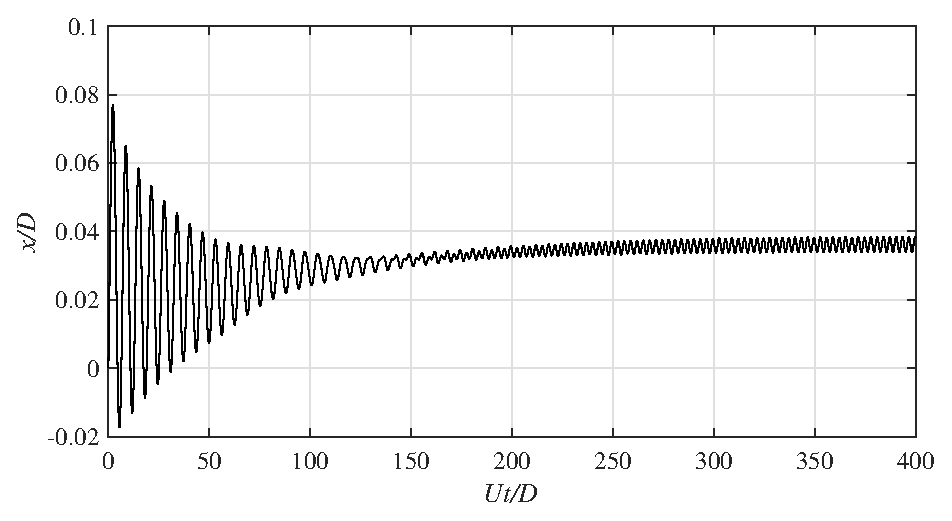
\includegraphics[width=\linewidth]{images/xdisp1.eps}
        \caption{$x$-component displacement}
     \end{subfigure}
    \begin{subfigure}[b]{0.6\linewidth}
        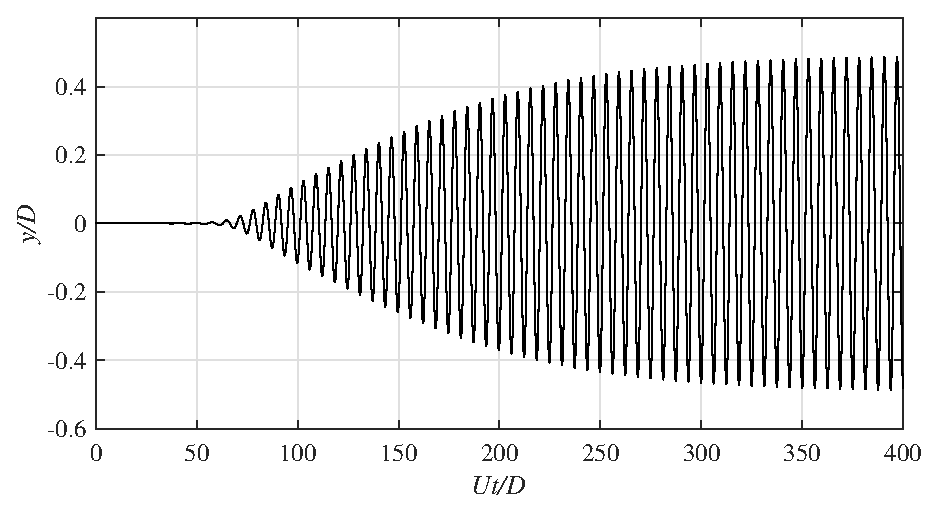
\includegraphics[width=\linewidth]{images/ydisp1.eps}
        \caption{$y$-component displacement}
    \end{subfigure}
      \caption{Time history of the displacement of the rigid circular cylinder}\label{results1}
\end{figure}

\section{VIV of a elastic circular cylinder}

\subsection{Case setup introduction}

This tutorial simulates the vortex-induced vibration of a three-dimensional (3D) elastic circular cylinder of the dimensions 10$D$ in length and $D$ in diameter. The cylinder can be viewed as an elastic beam with tension, compression, bending and torsional deformation capabilities. Without loss of generality, we divide the cylinder into twenty segments so that each segment has the length of $0.5D$. Both two ends of the cylinder are assigned with a fixed support. The cylinder is also assigned with a zero structural damping and low non-dimensional mass to encourage high-amplitude oscillations. Simulations are carried out on a 3D O-block mesh with a outer diameter $15D$ and $80\times80\times20$ finite volume cells. Grid points are uniform distributed in circumferential and spanwise directions, while in radical direction, the grid spacing follows from an exponential distribution with an exponential coefficient of 1.0478. 

\subsection{Procedure}

The detailed procedures of this tutorial are identical to the previous one, as well as most of the case files in these two tutorials. We now demonstrate the remaining differences between them. In the file blockMeshDict, the block entry now takes the form 

\begin{lstlisting}
blocks
(
    hex (1 4 10 7 0 5 11 6) (22 20 80) simpleGrading (1 1 40)
    hex (3 1 7 9 2 0 6 8) (22 20 80) simpleGrading (1 1 40)
    hex (4 3 9 10 5 2 8 11) (36 20 80) simpleGrading (1 1 40)
);
\end{lstlisting}

\noindent The types of the `front' and `back' patches are changed from empty to cyclic.

\begin{lstlisting}
    front
    {
        type cyclic;
        neighbourPatch back;
        faces
        (
            (0 5 4 1)
            (4 5 2 3)
            (3 2 0 1)
        );
    }
    back
    {
        type cyclic;
        neighbourPatch front;
        faces
        (
            (6 11 10 7)
            (10 11 8 9)
            (9 8 6 7)
        );
    }
\end{lstlisting}

\noindent In the file constant/dynamicMeshDict, the keyword `nNode' now takes the value of 21 considering the cylinder is divided into 20 segments. Meanwhile, the entry `length' (which takes a list of scalars as an input) now writes

\begin{lstlisting}
// Select "sixDoFElasticBodyMotion" for 6DoFs beams
motionSolver    sixDoFElasticBodyMotion;

// Number of nodes (an integer larger than 2) on the beam
nNode 21;

// Length of element segments (the number of elements should equal to $nNode minus 1)
length 20{0.5}
\end{lstlisting}

\noindent  Accordingly, the shape of the first mode, in which the cylinder undergoes a bending deflection in the $XZ$ plane, is expressed as 

\begin{lstlisting}
// The first mode (a list of six-component vectors for 6DoFs beams)
mode1 List<vector6D>
21
(
((0.000000 0 0) (0 0.000000 0))
((0.024472 0 0) (0 0.097081 0))
((0.095492 0 0) (0 0.184658 0))
((0.206107 0 0) (0 0.254160 0))
((0.345492 0 0) (0 0.298783 0))
((0.500000 0 0) (0 0.314159 0))
((0.654508 0 0) (0 0.298783 0))
((0.793893 0 0) (0 0.254160 0))
((0.904508 0 0) (0 0.184658 0))
((0.975528 0 0) (0 0.097081 0))
((1.000000 0 0) (0 0.000000 0))
((0.975528 0 0) (0 -0.097081 0))
((0.904508 0 0) (0 -0.184658 0))
((0.793893 0 0) (0 -0.254160 0))
((0.654508 0 0) (0 -0.298783 0))
((0.500000 0 0) (0 -0.314159 0))
((0.345492 0 0) (0 -0.298783 0))
((0.206107 0 0) (0 -0.254160 0))
((0.095492 0 0) (0 -0.184658 0))
((0.024472 0 0) (0 -0.097081 0))
((0.000000 0 0) (0 0.000000 0))
);
\end{lstlisting}

\noindent Similarly, the shape of the second mode takes the form

\begin{lstlisting}
// The second mode (a list of six-component vectors for 6DoFs beams)
mode2 List<vector6D>
21
(
((0 0.000000 0) (0.000000 0 0))
((0 0.024472 0) (-0.097081 0 0))
((0 0.095492 0) (-0.184658 0 0))
((0 0.206107 0) (-0.254160 0 0))
((0 0.345492 0) (-0.298783 0 0))
((0 0.500000 0) (-0.314159 0 0))
((0 0.654508 0) (-0.298783 0 0))
((0 0.793893 0) (-0.254160 0 0))
((0 0.904508 0) (-0.184658 0 0))
((0 0.975528 0) (-0.097081 0 0))
((0 1.000000 0) (0.000000 0 0))
((0 0.975528 0) (0.097081 0 0))
((0 0.904508 0) (0.184658 0 0))
((0 0.793893 0) (0.254160 0 0))
((0 0.654508 0) (0.298783 0 0))
((0 0.500000 0) (0.314159 0 0))
((0 0.345492 0) (0.298783 0 0))
((0 0.206107 0) (0.254160 0 0))
((0 0.095492 0) (0.184658 0 0))
((0 0.024472 0) (0.097081 0 0))
((0 0.000000 0) (0.000000 0 0))
);
\end{lstlisting}

Finally, one can quickly run this tutorial by executing the Allrun command in the terminal as shown below

\begin{quote}
\begin{verbatim}
$ ./Allrun
\end{verbatim}
\end{quote}

\subsection{Results}

Figure \ref{results2} plots the time history of the displacement of the elastic circular cylinder at its mid-point.

\begin{figure}[H]
\centering
    \begin{subfigure}[b]{0.6\linewidth}
        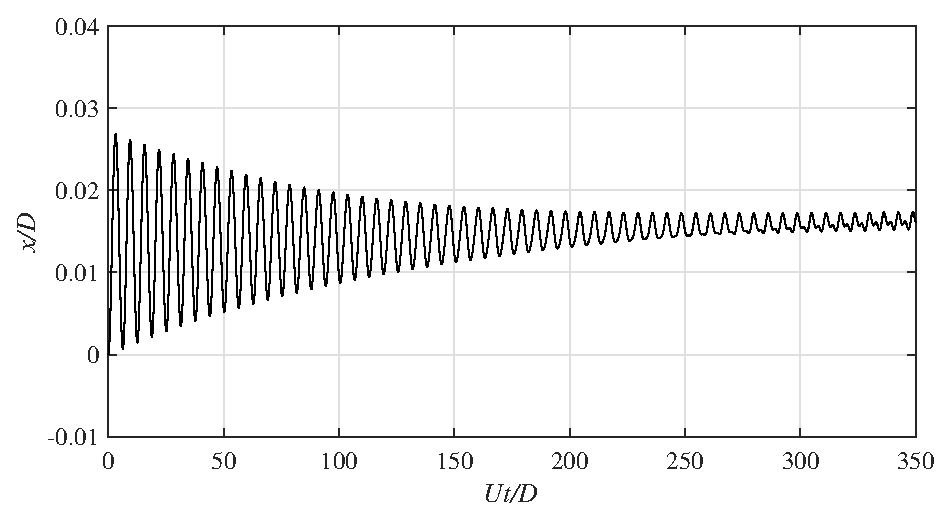
\includegraphics[width=\linewidth]{images/xdisp2.eps}
        \caption{$x$-component displacement}
     \end{subfigure}
    \begin{subfigure}[b]{0.6\linewidth}
        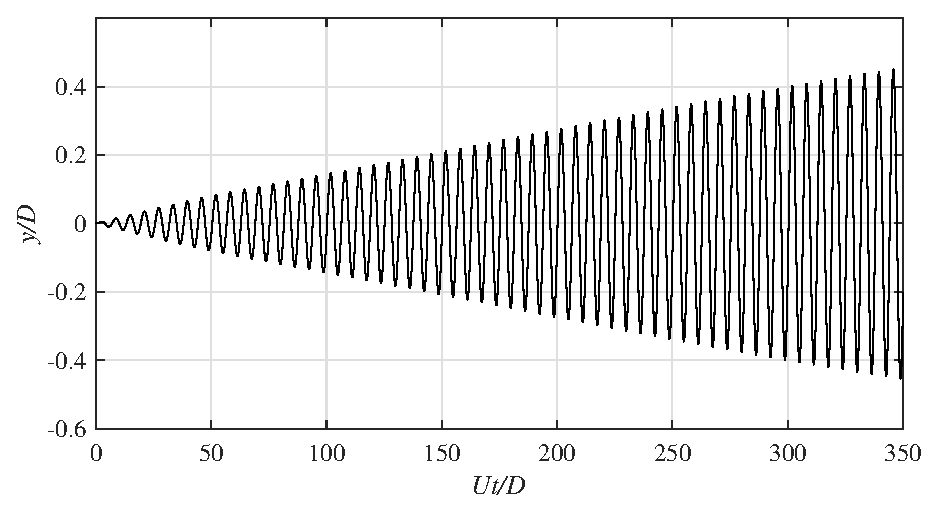
\includegraphics[width=\linewidth]{images/ydisp2.eps}
        \caption{$y$-component displacement}
    \end{subfigure}
      \caption{Time history of the displacement of the elastic circular cylinder at its mid-point}\label{results2}
\end{figure}


%\chapter{User Training}


% \appendix
% \chapter{More Monticello Candidates}

\pagestyle{plain}
{
  \renewcommand{\thispagestyle}[1]{}
  \printbibliography           
}

\end{document}
